\section{Implementaciones y cálculos}\label{sec:impl}
En esta sección daremos algunas evidencias computacionales de la estabilidad de los diagramas de persistencias, centrándonos filtraciones de complejos simpliciales asociadas a nubes de puntos con un cierto ruido. Para ello comenzaremos estudiando posibles algoritmos para calcular tanto la \emph{distancia Hausdorff} como la \emph{distancia bottleneck}. 
\subsection{Cálculo de la distancia Hausdorff}

\begin{definition}
Sea $A$ y $B$ dos conjuntos de puntos. Se define la \emph{distancia Hausdorff directa} entre $A$ y $B$ como el máximo de las distancias entre cada punto $x \in A$ y el punto $y \in B$ más cercano a $x$. Es decir,
\[
\check{H}(A,B)= \adjustlimits\sup_{x \in A} \inf_{y \in B} \norm{x-y}_\infty\,.
\]
\end{definition}

\begin{remark}
$\check{H}(A,B) \neq \check{H}(B,A)$ y por tanto la distancia Hausdorff directa no es simétrica.
\end{remark}

Luego, la distancia de Hausdorff es el máximo de las distancias Hausdorff directas en ambas direcciones, es decir
\[
H(A,B) = \max\{\check{H}(A,B), \check{H}(B,A)\}\,.
\]

Sea $A=\{x_1, x_2, ...,x_m\}$ y $B=\{y_1, y_2, ...,y_m\}$ los dos conjuntos de puntos en $\mathbb{R}^k$ y sea $\norm{x-y}_\infty$ la distancia infinito entre $x$ e $y$. Por lo tanto, podemos calcular de manera sencilla la distancia Hausdorff directa entre $A$ y $B$ de la siguiendo los pasos del algoritmo \ref{ref:HausdorffDirect}.

\begin{algorithm}[!ht]
\caption{Cálculo de la distancia Hausdorff directa}\label{ref:HausdorffDirect}
\begin{algorithmic}[1]
\Require Dos conjuntos finitos de puntos $A$ y $B$
\Ensure Distancia Hausdorff directa entre $A$ y $B$
\State $cmax\gets 0$
\For{$x \in A$}
	\State $cmin\gets \infty$
	\For{$y \in B$}\Comment{Calculamos $d_\infty(x, B)=\inf_{y \in B} d_\infty(x,y)$}
		\State $d\gets \norm{x-y}_\infty$
		\If{$d < cmin$}
			\State $cmin\gets d$
		\EndIf
	\EndFor
	\If{$cmin > cmax$}\Comment{Recalculamos el supremo}
		\State $cmax\gets cmin$
	\EndIf
\EndFor
\State \textbf{return} $cmax$
\end{algorithmic}
\end{algorithm}

Obviamente, la complejidad del algoritmo \ref{ref:HausdorffDirect} es del orden de $\bigO(n*m)$, donde $m = \abs{A}$ y $n = \abs{B}$. La distancia Hausdorff entre $A$ y $B$  será el máximo de los resultados de ejecutar el algoritmo \ref{ref:HausdorffDirect} en ambas direcciones, y por lo tanto la complejidad de calcular la distancia Hausdorff de este modo es de $\bigO(n*m)$.

Sin embargo, existen implementaciones del cálculo de la distancia Hausdorff que tienen complejidad del orden de $\bigO(m)$ en el mejor de los casos y $\bigO(n*m)$ en el peor de los casos \cite{ArticuloHausdorff}.
\subsection{Cálculo de la distancia bottleneck}
En esta sección veremos los algoritmos propuestos en \cite{libroEH}, donde el cálculo de la distancia bottleneck entre dos diagramas de persistencia se reduce a la obtención de un emparejamiento óptimo en un grafo bipartido.

\subsubsection*{Obtención de la distancia a partir de emparejamientos}
Empezaremos viendo cómo podemos obtener la distancia bottleneck entre diagramas de persistencia a partir de emparejamientos de un grafo bipartido.

Sea $X$ e $Y$ dos diagramas de persistencia, para los que asumimos que están formados por un número finito de puntos fuera de la diagonal e infinitos puntos en ella. Denotamos $X_0$ al multiconjunto finito de los puntos fuera de la diagonal en $X$ y $X_0'$ a la proyección ortogonal de $X_0$ sobre la diagonal. Por tanto, construimos el grafo bipartido completo
\[
G= (U \cupdot V, A), \text{ con } U=X_0 \cupdot Y_0', V=Y_0 \cupdot X_0', \text{ y } A=U\times V\,,
\]
donde $U \cupdot V$ denota la unión disjunta de los conjuntos $U$ y $V$.

En este grafo introducimos la función de coste $c: A \to \mathbb{R}$ donde a cada arista $uv \in A$ se le asigna la la distancia infinito entre los puntos $u$ y $v$:
\[
c(uv)=
\begin{cases}
\norm{u-v}_\infty & \text{ si } u \in X_0 \text{ ó } v \in Y_0   \\ 
0 & \text{ si } u \in Y_0' \text{ y } v \in X_0' 
\end{cases}
\]

\begin{remark}
Por construcción, la arista de coste mínimo que conecta un punto $u$ fuera de la diagonal con un punto de la diagonal es $uu'$, donde $u'$ es la proyección ortogonal de $u$ sobre la diagonal. Además, el coste de esta arista es la mitad de la persistencia de $u$. 
\end{remark}

\begin{definition}
Un \emph{emparejamiento} en $G$ es un subconjunto $M \subseteq A$ tal que dos aristas de $M$ no tienen un vértice en común. Diremos que
\begin{itemize}
	\item $M$ es \emph{maximal} si no existe un emparejamiento $M'$ en $G$ con $M \subset M'$.
	\item $M$ es \emph{máximo} si no existe un emparejamiento $M'$ en $G$ con $\text{card } M < \text{card } M'$.
	\item $M$ es \emph{perfecto} si todos los vértices de $G$ son extremo de alguna arista de $M$.
\end{itemize}
\end{definition}

Como $G$ es un grafo bipartido completo, todo emparejamiento máximo es también un emparejamiento perfecto.

\begin{definition}
Se define $G(\epsilon)=(U \cupdot V, A_\epsilon)$ como el subgrafo de $G$ que se obtiene al eliminar todas las aristas $uv \in A$ con coste $c(uv)>\epsilon$.  
\end{definition}
En este caso, todo emparejamiento perfecto en $G(\epsilon)$ es máximo, sin embargo, el opuesto no siempre es cierto.

\begin{definition}
Un \emph{emparejamiento de coste mínimo} es un emparejamiento máximo que minimiza la suma de los costes de las aristas del emparejamiento. Denotaremos a esta suma como el \emph{coste total} del emparejamiento.
\end{definition}

\begin{lemma}[Lema de reducción {\cite[Chapter~8]{libroEH}}]
Sean $X$ e $Y$ dos diagramas de persistencia y sea $G =(U \cupdot V, A)$ su correspondiente grafo bipartido. Entonces la distancia bottleneck entre $X$ e $Y$ es el menor $\epsilon$ tal que el subgrafo $G(\epsilon)$ tiene un emparejamiento perfecto.
\end{lemma}

Por lo tanto, el cálculo de la distancia bottleneck entre diagramas de persistencia se reduce a la obtención de emparejamientos perfectos con coste mínimo en grafos bipartidos.

\subsubsection*{Emparejamientos en grafos bipartidos}
Comenzaremos viendo cómo podemos obtener emparejamientos máximos en el grafo bipartido $G(\epsilon)=(U \cupdot V, A_\epsilon)$. Para ello haremos uso de algoritmos iterativos, donde en cada paso mejoraremos el emparejamiento, hasta que no sea posible aumentarlo.

\begin{definition}
Sea $M_i$ el emparejamiento tras realizar $i$ iteraciones. Se define $D_i = (P, Q)$ como el digrafo tal que
\begin{itemize}
	\item $P= (U \cupdot V) \cup \{s, t\}$, donde $s$ se denota como fuente y $t$ como sumidero.
	\item $Q = Q_1 \cup Q_2$, donde 
	\begin{itemize}
		\item $Q_1$ son las aristas $x \in A_\epsilon$ tal que $x$ va de $V$ a $U$ si pertenece al emparejamiento $M_i$, y $x$ va de $U$ a $V$ en caso contrario.
		\item $Q_2$ son las aristas que van desde $s$ a los vértices no emparejados $u \in U$, más las aristas que van desde los vértices no emparejados $v \in V$ a $t$.
	\end{itemize}
\end{itemize}

\end{definition}

En la figura \ref{ref:ejEmparejamiento} podemos observar un ejemplo del digrafo $D_i$ asociado a un emparejamiento $M_i$.

\begin{figure}[!ht]
\centering
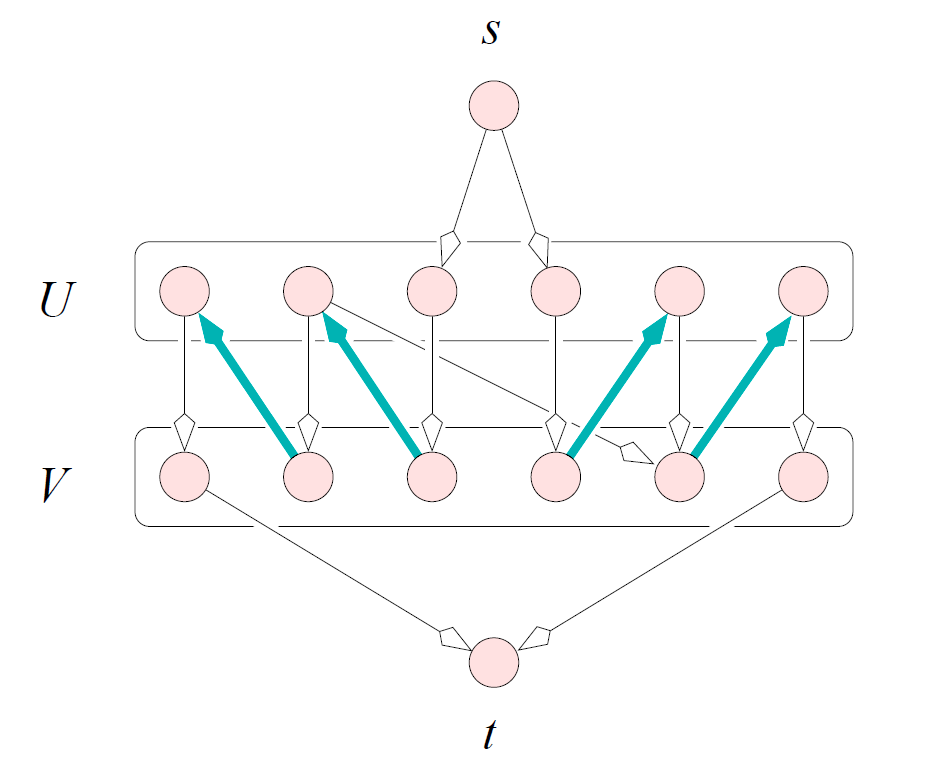
\includegraphics[width=0.5\textwidth]{include/figuras/emparejamiento.png} 
\caption{Digrafo asociado a un emparejamiento de cuatro aristas. Fuente: \cite{libroEH}}
\label{ref:ejEmparejamiento}
\end{figure}  

\begin{definition}
Un \emph{camino de $M_i$-aumento} es un camino dirigido desde $s$ hasta $t$ el cual visita un vértice de $D_i$ como máximo una vez.
\end{definition}

Claramente, si tenemos un camino de $M_i$-aumento con $k$ vértices no contenidos en $M_i$ y $k-1$ vértices en $M_i$, entonces podemos mejorar el emparejamiento sustituyendo los $k$ vértices que no estaban en $M_i$ por los $k-1$ vértices que si estaban en $M_i$. Cuando hacemos esta mejora, decimos que hemos \emph{aumentado} el emparejamiento usando el camino. 

\begin{lemma}[Lema de Berge]
$M_i$ es un emparejamiento máximo de $G(\epsilon)$ si y sólo si $G(\epsilon)$ no contiene caminos de $M_i$-aumento.
\end{lemma}

Luego, para obtener un emparejamiento máximo de $G(\epsilon)$ seguiremos los siguientes pasos:

\begin{algorithm}[!ht]
\caption{Obtención de emparejamientos máximos}\label{ref:algEmpMax}
\begin{algorithmic}[1]
\Require $G(\epsilon)=(U \cupdot V, A_\epsilon)$ grafo bipartido
\Ensure $M_i$ es un emparejamiento máximo de $G(\epsilon)$
\State $M_0\gets \emptyset$
\State $i\gets 0$
\While{existe un camino de $M_i$-aumento en $D_i$}
	\State aumentar $M_i$ usando el camino para obtener $M_{i+1}$
	\State $i\gets i+1$
\EndWhile
\State \textbf{return} $M_i$
\end{algorithmic}
\end{algorithm}

Este algoritmo terminará como mucho en $n$ iteraciones, siendo $n= \text{card } U = \text{card } V$, ya que en cada iteración se aumenta el tamaño del emparejamiento en uno. Podemos hacer uso de la \emph{búsqueda en anchura} y la \emph{búsqueda en profundidad} para encontrar caminos de $M_i$-aumento en un tiempo proporcional al número de aristas en $A_\epsilon$. Por lo que la complejidad del algoritmo es del orden de $\bigO(n^3)$.

Se puede obtener una complejidad del orden de $\bigO(n^{5/2})$ implementando el algoritmo que se muestra en \cite{libroEH}. Este hace uso de la \emph{búsqueda en anchura} para etiquetar los vértices con su distancia a $s$ y después usa la \emph{búsqueda en profundidad} para construir un conjunto maximal de múltiples caminos de $M_i$-aumento.  

\subsubsection*{Emparejamientos de coste mínimo en grafos bipartidos}
Para calcular el menor $\epsilon$ tal que $G(\epsilon)$ tiene un emparejamiento perfecto, seguiremos una variante del método húngaro, el cual se utiliza para resolver problemas de asignación \cite{metodoHungaro}. 

\begin{property}[{\cite[Chapter~8]{libroEH}}]
\leavevmode
\begin{enumerate}
	\item Si el subgrafo $G(0)$, que consiste en las aristas de coste cero de $G$, tiene un emparejamiento perfecto, entonces es un emparejamiento de coste mínimo. Es más, su coste total es cero.
	\item Restar la misma cantidad al coste de todas las aristas incidentes a un vértice de $G$ afecta a todos los emparejamientos perfectos de la misma forma. En particular, un emparejamiento perfecto minimiza el coste total antes de las restas de las cantidades si y sólo si sigue minimizándolo tras las restas de las cantidades.
\end{enumerate}
\end{property}

Así pues, empezaremos construyendo un emparejamiento máximo en $G(0)$. Si es un emparejamiento perfecto ya hemos acabado y por lo tanto la distancia bottleneck entre los diagramas de persistencia es $0$. En otro caso, cambiaremos los costes de las aristas de $G$ preservando el orden de los emparejamientos perfectos en $G$ por coste total. Para ello introducimos las \emph{funciones de reducción} $d_i: U \times V \to \mathbb{R}$. Partiendo de $d_0(x)=0$ para todos los vértices de $G$, el algoritmo cambiará el valor de la función de reducción en cada iteración $i$.

\begin{definition}
Sea $c(xy)$ el coste original de la arista $xy \in G$. Se define el \emph{coste modificado} tras $i$ iteraciones como
\[
c_i(xy) = c(xy) - d_i(x) - d_i(y) > 0\,.
\]
\end{definition}

Sea $G_i$ el grafo $G$ con los costes modificados por $d_i$, entonces el algoritmo construirá iterativamente emparejamientos máximos en $G_i(0)$, que coincide con el subgrafo resultante al eliminar las aristas con peso no nulo de $G_i$. Incrementando el número de aristas del emparejamiento máximo en uno por cada iteración, obtendremos el emparejamiento perfecto en $n$ iteraciones.

Análogo al método Húngaro, iremos añadiendo aristas de coste modificado cero al emparejamiento en cada iteración y para generar ceros adicionales en los costes modificados de las aristas seleccionaremos el menor de los costes totales de los caminos de $M_i$-aumento como cantidad que variará la función de reducción.

Sea $M_i$ un emparejamiento máximo en $G_i(0)$ y sea $D_i$ el digrafo asociado al emparejamiento $M_i$ y $G_i$. Si $M_i$ no es un emparejamiento perfecto en $G_i$, entonces no es un emparejamiento máximo en $G_i$, y por lo tanto existirá un camino de $M_i$-aumento en $D_i$.

Por definición $c_i(sy) = c_i(xt) = 0$ para todo $x \in U$ e $y \in V$. Se denota como \emph{coste total} de un camino de $M_i$-aumento como la suma de los costes modificados de sus aristas. Obtendremos el camino de $M_i$-aumento $\pi$ que minimiza el coste total, a través del \emph{algoritmo de Dijkstra} con una complejidad del orden de $\bigO(n^2)$.

Como hacíamos en el algoritmo \ref{ref:algEmpMax}, aumentamos $M_i$ usando $\pi$ para obtener $M_{i+1}$. Vamos a garantizar que podemos cambiar la función de reducción de forma que todas las aristas del emparejamiento $M_{i+1}$ tienen coste modificado cero. Para ello definimos $\gamma_i(x)$ como el coste total mínimo de los caminos desde $s$ hasta $x$.

De esta forma, actualizamos las funciones de reducción a
\[
d_{i+1} = \begin{cases}
d_i(x) - \gamma_i(x) & \text{ si } x \in U \\ 
d_i(x) + \gamma_i(x) & \text{ si } x \in V 
\end{cases}
\]
Luego, para todos los vértices $u \in U$ y $v \in V$, el nuevo coste modificado de la arista $uv$ es:
\[
c_{i+1}(uv)=c(uv) - d_i(u) - d_i(v) + \gamma_i(u) - \gamma_i(v)\,.
\]

%TODO Añadir demostración
\begin{property}[{\cite[Chapter~8]{libroEH}}]
Sea $M_{i+1}$ el emparejamiento máximo obtenido al aumentar $M_i$. Entonces, $c_{i+1}(uv) \geq 0$ para toda arista $uv$ en $G_i$, y  $c_{i+1}(uv) = 0$ para toda arista $uv \in M_{i+1}$.
\end{property}

La propiedad anterior garantiza que en la última iteración obtenemos el emparejamiento perfecto de coste total mínimo, y por tanto la distancia bottleneck entre los diagramas de persistencia $X$ e $Y$ es igual al máximo de los costes originales de las aristas de dicho emparejamiento perfecto, es decir
\[
W_\infty(X,Y)=\max_{xy \in M_n} c(xy),\text{ siendo } n= \text{card } U = \text{card } V\,.
\]
Como tenemos $n$ iteraciones en las cuales cada una aplicamos el algoritmo de Dijkstra, entonces la complejidad del cálculo de la distancia bottleneck siguiendo el algoritmo comentado es del orden de $\bigO(n^3)$.

\subsection{Pruebas}
La implementación del cálculo de las distancias se ha realizado en Python y el código se puede encontrar en el Anexo \ref{codigo_dist}. Para ello he utilizado la librería GUDHI para los cálculos de los alfa complejos \cite{gudhi:AlphaComplex}, complejos de Vietoris-Rips \cite{gudhi:RipsComplex} y la persistencia \cite{gudhi:PersistenceRepresentations}.

Para comprobar el resultado del problema estudiaremos la robustez de los diagramas de persistencia para un conjunto finito de puntos y una variación de dicho conjunto dada por un cierto ruido. Obtendremos filtraciones de alfa complejos para ambos conjuntos de puntos, y calcularemos la distancia bottleneck entre sus diagramas de persistencia. Veremos que para el caso de los alfa complejos de nubes de puntos obtenemos el siguiente teorema de estabilidad

\begin{theorem}[Teorema de estabilidad para alfa complejos de nubes de puntos]\label{th:estabilidadAlfa}
Sean $A$ y $B$ subconjuntos finitos de $\mathbb{R}^d$ y $\text{\rm Dgm}_k(A)$ el diagrama de persistencia de dimensión $k$ de las filtraciones del alfa complejo asociado a $A$. Entonces, para cada $k$
\[
W_\infty(\text{\rm Dgm}_k(A), \text{\rm Dgm}_k(B)) \leq H(A, B)\,.
\]
\end{theorem}

Para su demostración haremos uso de los siguientes resultados:

\begin{theorem}[Teorema de la invariancia homotópica {\cite[Theorem~2.10]{Hatcher}}]
\begin{sloppypar}
Si dos funciones $f, g: X \to Y$ son homotópicas, entonces inducen el mismo homomorfismo  ${f_*=g_*:\text{\rm H}_n(X) \to \text{\rm H}_n(X)}\,$.
\end{sloppypar}
\end{theorem}
Y su correspondiente corolario,
\begin{corollary}[{\cite[Corollary 2.11]{Hatcher}}]\label{cor:homotopia}
Las funciones $f_*:\text{\rm H}_n(X) \to \text{\rm H}_n(X)$ inducidas por la equivalencia homotópica $f:X \to Y$, son isomorfismos para todo $n$.
\end{corollary}

\begin{proof}[Demostración del Teorema \ref{th:estabilidadAlfa}]
Sean $d^A: \mathbb{R}^d \to \mathbb{R}$ la función que asigna a cada punto $p \in \mathbb{R}^d$ su distancia a $A$, $x \in \mathbb{R}^d$ un punto y supongamos que $d^A(x) \leq d^B(x)$. Utilizando la desigualdad triangular se sigue que
\[
d^A(x) \leq H(A,B) + d^B(x) \text{ por lo que } d^A(x) - d^B(x) \leq H(A,B)\,.
\] 

Análogamente, si $d^B(x) \leq d^A(x)$ se sigue que $d^B(x) - d^A(x) \leq H(A,B)$ por lo que
\[
\norm{d^A- d^B}_\infty \leq H(A,B)\,.
\] 

Por otro lado, la definición de la distancia Hausdorff y el hecho de que $A$ y $B$ sean compactos garantiza que extisten $x\in A$ e $y \in B$ tal que $H(A,B)=\max\{d^A(y), d^B(x)\}$, pero
\begin{gather*}
d^A(y) = \abs{d^A(y) - d^B(y)} \leq \norm{d^A - d^B}_\infty\,,\\
d^B(x) = \abs{d^A(x) - d^B(x)} \leq \norm{d^A - d^B}_\infty\,.
\end{gather*}
Por tanto $H(A,B) = \norm{d^A - d^B}_\infty\,.$

\begin{figure}[!ht]
\centering
\begin{subfigure}{0.45\textwidth}
\centering
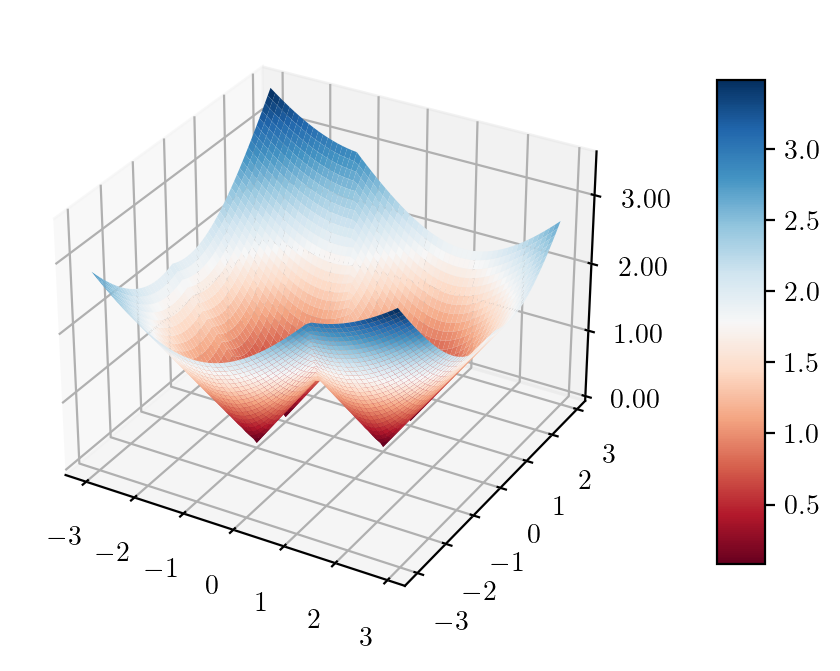
\includegraphics[width=\textwidth]{../code/output/grafoDistancias.png} 
\caption{Reprsentación del grafo de $d^A$ en $\mathbb{R}^3$.}
\label{ref:grafoDistConj}
\end{subfigure}\hspace{0.1\textwidth}%
\begin{subfigure}{0.45\textwidth}
\centering
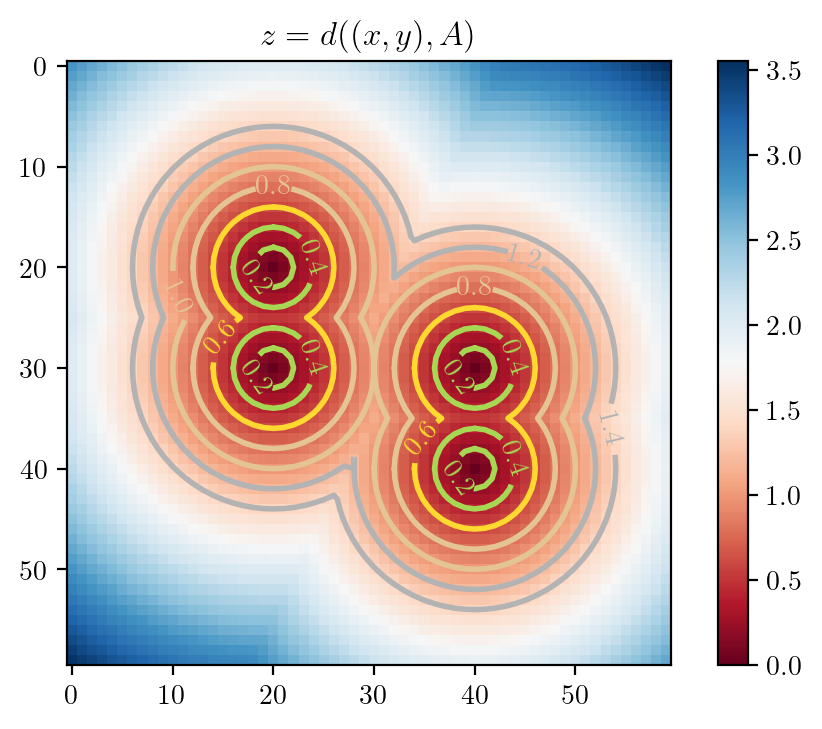
\includegraphics[width=\textwidth]{../code/output/subnivelDistancias.png} 
\caption{Representación de los conjuntos de subnivel $\widehat{L}_r$.}
\label{ref:subnivelDistConj}
\end{subfigure}
\caption{Grafo de $d^A$ y sus conjuntos de subnivel, siendo el conjunto de puntos $A = \{(-1, 0), (1, 0), (1, 1), (-1, -1)\}\,$. El código para la obtención de las figuras se encuentra en el Anexo \ref{codigo_vis_dist}.}
\label{ref:figDistConj}
\end{figure}

Además, si denotamos al conjunto de subnivel $\widehat{L}_\epsilon=\{x \mid d^A \leq \epsilon\}$, que es la unión de las bolas cerradas centradas en los puntos de $A$ y radio $\epsilon$, como podemos ver en la figura \ref{ref:figDistConj}. Como consecuencia del \emph{Lema del Nervio} $\text{H}_k(\widehat{L}_r) \cong \text{H}_k(\text{\v{C}ech}(r))$, para todo $k$ debido a que el complejo de \v{C}ech tiene el mismo tipo de homotopía que la unión de las bolas cerradas de radio $r$ centradas en los puntos de $A$.

Y como el complejo de \v{C}ech tiene el mismo tipo de homotopía que el alfa complejo entonces, como consecuencia del corolario \ref{cor:homotopia},

\[
\text{H}_k(\text{Alpha}(r)) \cong \text{H}_k(\text{\v{C}ech}(r)) \cong \text{H}_k(\widehat{L}_r), \text{ para todo } k\,.
\]
\end{proof}

El código de las siguientes pruebas se puede encontrar en el Anexo \ref{codigo_ej}.

\subsubsection{Ejemplo 1: Elipse}
Empezaremos viendo un ejemplo sencillo de la curva de una elipse dada por la siguiente parametrización:
\[
\gamma(t)= (4\sin(t), 9\cos(t)), \text{ con } t\in [0,2\pi]
\]

De esta curva obtenemos 30 puntos y obtenemos las filtraciones de alfa complejos asociadas a dichos puntos. Además, introducimos una pequeña cantidad de ruido en los puntos a través de una distribución normal $N(2, 0.09)$, y obtenemos sus filtraciones de alfa complejos asociadas. Una vez obtenidas las filtraciones obtendremos los diagramas de persistencia correspondientes como se muestra en la figura \ref{ref:persEj1}.

\begin{figure}[!ht]
\centering
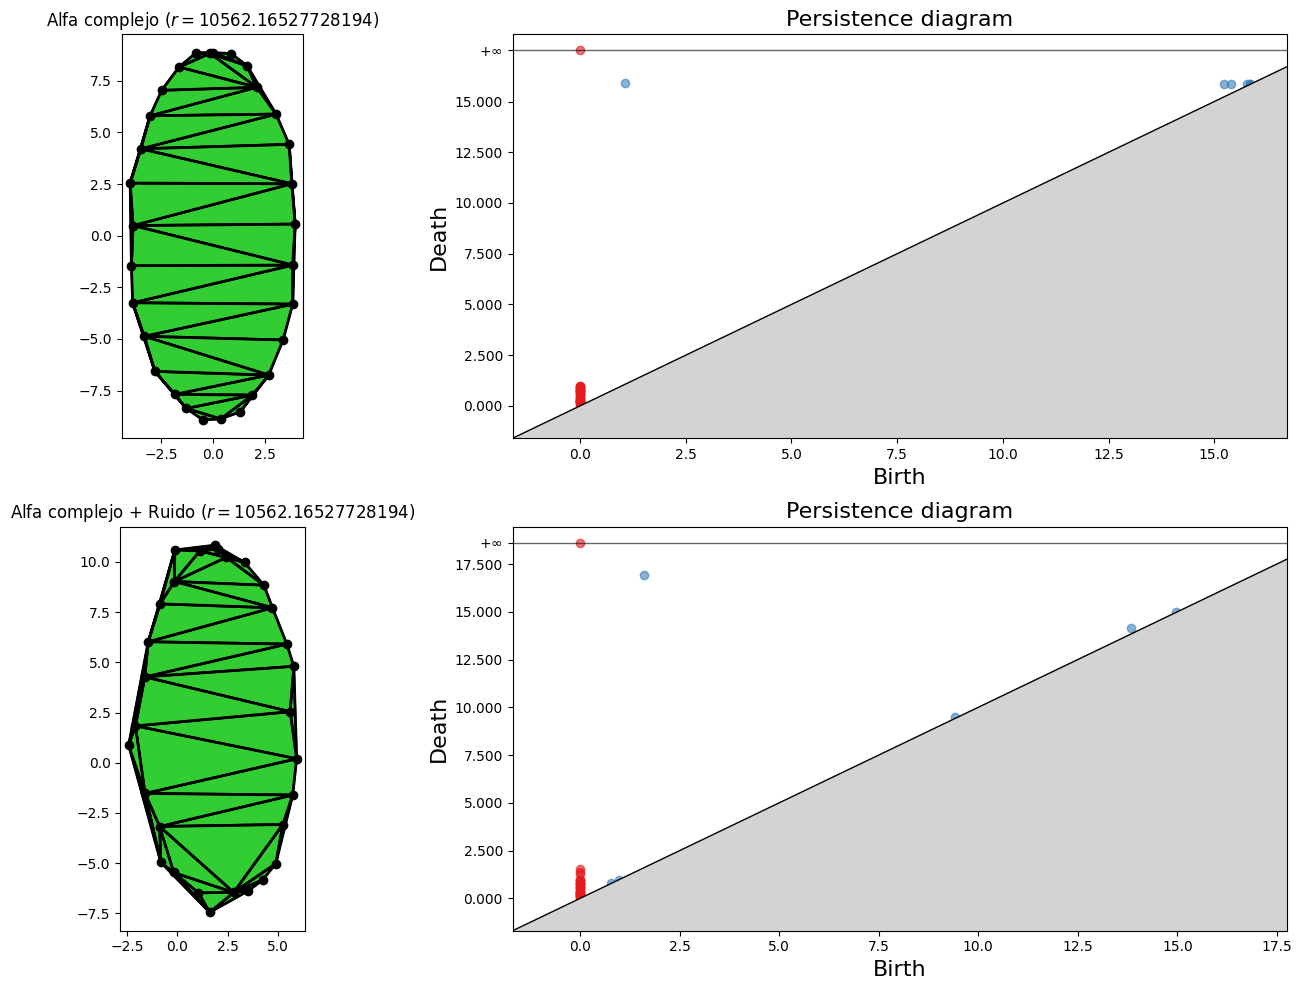
\includegraphics[width=\textwidth]{../code/output/ejemplo1.png} 
\caption{Alfa complejos y diagramas de persistencias asociados a las filtraciones de los alfa complejos. En las figuras superiores se toma como entrada una elipse y en las inferiores la misma elipse más cierto ruido.}
\label{ref:persEj1}
\end{figure} 

Podemos observar a simple vista en la figura \ref{ref:persEj1} que los diagramas de persistencia varían poco, y las características más importantes se mantienen. Se ve que en ambos diagramas para la dimensión cero la mayoría de las clases mueren muy pronto y una de ellas nunca muere, lo que refleja que la elipse es conexa. Por otro lado, en las clases de dimensión 1 todas están muy cercanas a la diagonal excepto una que se mantiene durante un largo periodo de tiempo, lo cual refleja el agujero que contiene el interior de la elipse.

Esta similitud entre los diagramas queda demostrada al calcular la distancia bottleneck entre ellos para las dos dimensiones. Adicionalmente, se puede observar que se cumple el \emph{Teorema de estabilidad} debido a que la distancia bottleneck es inferior a la distancia Hausdorff entre los conjuntos de puntos, es decir, la variación entre los diagramas es inferior a la variación entre los puntos de la curva.

\begin{minipage}{\linewidth}
\consola{Ejemplo1}
\end{minipage}

\subsubsection{Ejemplo 2: Rosa polar}
Continuaremos viendo un ejemplo un poco más elaborado. Tomaremos la curva de una rosa polar dada por la siguiente parametrización:
\[
\alpha(t)= (10\cos(2t)\cos(t), 10\cos(2t)\cos(t)), \text{ con } t\in [0,2\pi]
\]

De esta curva obtenemos 50 puntos y obtenemos las filtraciones de alfa complejos asociadas a dichos puntos. En este caso introducimos una cantidad de ruido en los puntos superior respecto al anterior ejemplo. Estas perturbaciones se generan a través de una distribución normal $N(2, 0.25)$. Nuevamente, obtenemos sus filtraciones de alfa complejos asociadas a estos puntos. Una vez obtenidas las filtraciones obtendremos los diagramas de persistencia correspondientes como se muestra en la figura \ref{ref:persEj2}.

\begin{figure}[!ht]
\centering
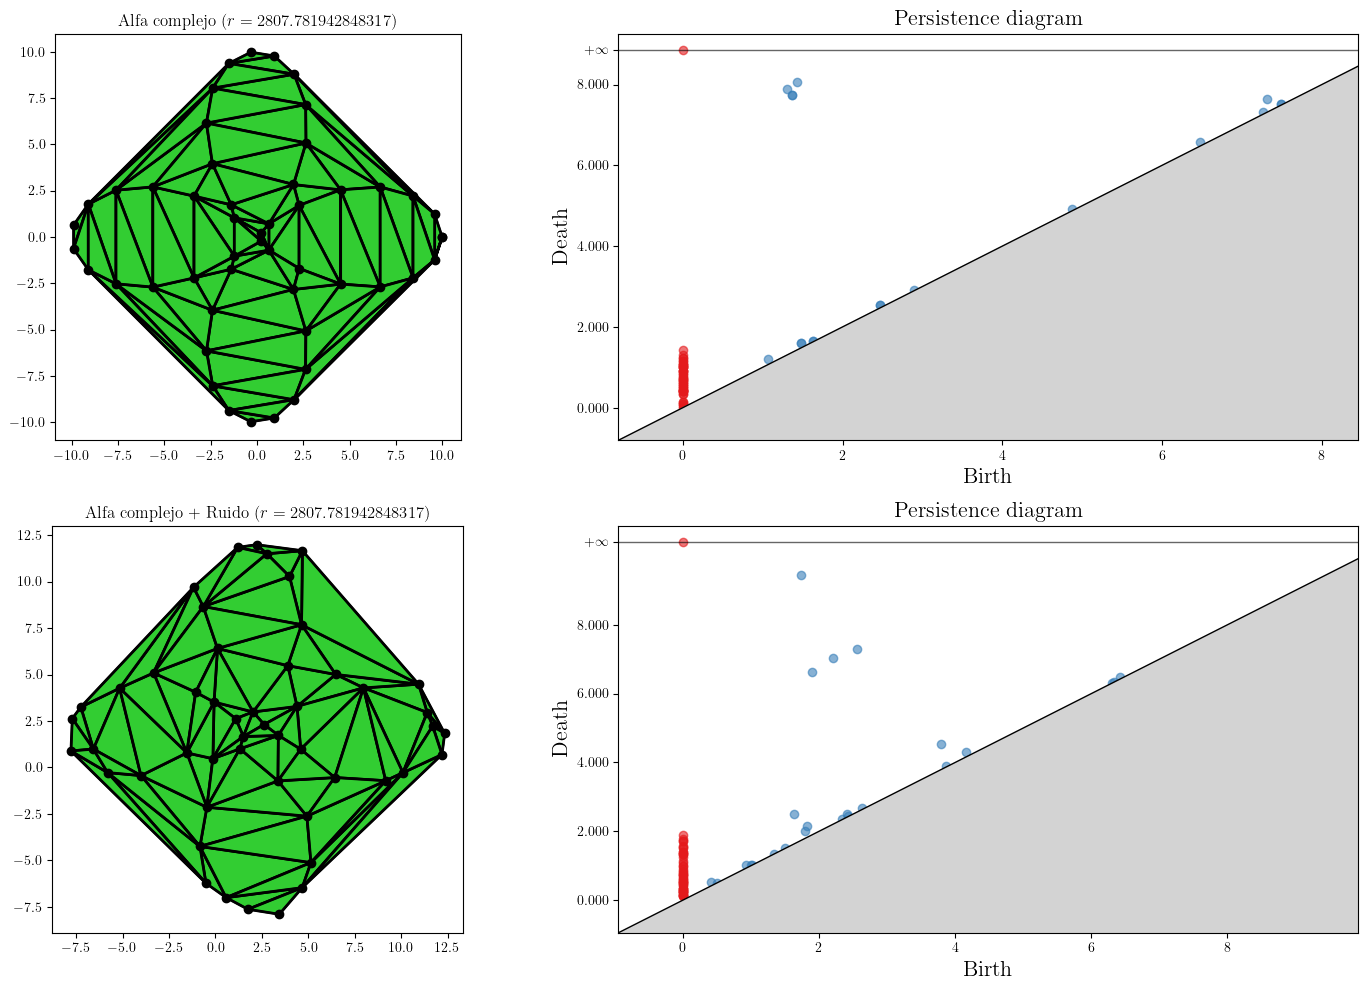
\includegraphics[width=\textwidth]{../code/output/ejemplo2.png} 
\caption{Alfa complejos y diagramas de persistencias asociados a las filtraciones de los alfa complejos. En las figuras superiores se toma como entrada una rosa polar y en las inferiores la misma rosa polar más cierto ruido.}
\label{ref:persEj2}
\end{figure} 

De nuevo, podemos observar a simple vista en la figura \ref{ref:persEj2} que los diagramas de persistencia varían poco, y las características más importantes se mantienen. Se ve que en ambos diagramas para la dimensión cero la mayoría de las clases mueren muy pronto y una de ellas nunca muere, lo que refleja que la rosa polar es conexa. Por otro lado, en las clases de dimensión 1 se observa que únicamente hay 4 clases en cada diagrama que se encuentran lejos de la diagonal, lo que refleja los 4 agujeros de esta rosa polar.

Cabe destacar que para el conjunto de datos inicial, estas cuatro clases mueren y nacen en momentos similares. Esto se debe a que, como podemos ver en la figura, los agujeros están bien definidos. Mientras que en el caso de los datos perturbados estos agujeros no se ven tan claros, lo cual se refleja en el diagrama al ver que 3 de los cuatros puntos comentados se encuentran mucho más cercanos a la diagonal.

Estas diferencias comentadas se pueden ver en el cálculo de la distancia bottleneck, ya que se observa que en la dimensión 1 tenemos una distancia superior que en el ejemplo anterior. Sin embargo, se observa que la distancia bottleneck es inferior a la distancia Hausdorff entre los conjuntos de puntos, dando lugar a la robustez que nos garantiza el \emph{Teorema de estabilidad}.

\consola{Ejemplo2}

\begin{remark}
En los ejemplos se indica la distancia bottleneck calculada tanto por mi implementación como la implementación de la librería GUDHI \cite{gudhi:BottleneckDistance} para poder garantizar que está bien calculada, ya que se ha observado que mi implementación obtiene erróneamente el resultado en algunas ocasiones. Esto se debe a que como hemos visto en los dos últimos ejemplos. los puntos de los diagramas se encuentran muy cercanos los unos a los otros en algunas ocasiones, lo que ocasiona en distancias de orden inferior a la precisión del tipo \textit{float}. Esto causa que se arrastren errores de número máquina a lo largo del proceso, ocasionando que se calculen erróneamente las distancias con el algoritmo de Dijkstra y por tanto que se obtenga un emparejamiento que no sea mínimo. 
\end{remark}

\subsubsection{Ejemplo 3: Elecciones generales noviembre 2019}
Por último, veremos un caso más práctico. Para ello simulamos el procedimiento descrito en \cite{votosArticulo}, donde se estudia cómo se puede hacer uso de la homología persistente para poder determinar si hay distritos electorales donde se ha votado diferente respecto al resto de distritos que lo rodean. Este tipo de estudio nos permitiría poder observar a gran escala si los votos condados en los condados son uniformes, o bien hay zonas donde se vota diferente.

Como se comenta en \cite{votosArticulo}, este trabajo es especialmente adecuada para la homología persistente, ya que identificaremos condados con ``distritos isla'' como agujeros. Para ello a cada distrito se le asigna una coordenada y en el caso de Estados Unidos se le asigna un color representando el partido ganador (rojo republicano y azul demócrata). En dicho artículo se plantean diversos complejos simpliciales y sus ventajas e inconvenientes para este tipo de tarea.

Así pues, he recreado este estudio para el caso de las elecciones generales del noviembre de 2019, donde he marcado a cada provincia del color del partido que obtuvo más votos en dicha región (datos en la tabla \ref{tab:ProvinciaPartido} del anexo). Nuestro interés desde el punto de vista de la estabilidad es poder garantizar que los resultados obtenidos en \cite{votosArticulo} son robustos independientemente de la coordenada elegida como representante de cada distrito/provincia.

Una vez obtenido el mapa toca decidir qué coordenadas se toman para cada una de las provincias. Como coordenadas ``canonicas'' he usado las coordenadas que aparecen en la página de la Wikipedia de cada una de las provincias. Y como datos perturbados he elegido unas coordenadas arbitrarias de cada una de las provincias. Estas coordenadas se pueden ver en la tabla \ref{tab:ProvinciaWiki} y \ref{tab:ProvinciaRand} del anexo.

Cabe destacar que en este ejemplo no se han utilizado filtraciones de alfa complejos para obtener los diagramas de persistencia, sino que se han utilizado filtraciones de complejos de Vietoris-Rips. Esto se debe a que los alfa complejos requieren que los puntos se encuentren en posición general para obtener el complejo de Delaunay, lo cual podía no ocurrir al elegir puntos aleatorios.

Sin embargo, el siguiente corolario del teorema \cite[Theorem~5.2]{persistenciaRips} nos garantiza la estabilidad para los diagramas de persistencia asociado a filtraciones de complejos de Vietoris-Rips:

\begin{corollary}[Teorema de estabilidad para complejos de Vietoris-Rips de espacios métricos acotados]
$ $\\
Sean $X, Y$ dos espacios métricos acotados y $\text{\rm Dgm}_k(X)$ el diagrama de persistencia de dimensión $k$ de las filtraciones del complejo de Vietoris-Rips asociado a $X$. Entonces, para cada $k$
\[
W_\infty(\text{\rm Dgm}_k(X), \text{\rm Dgm}_k(Y)) \leq H(X, Y)\,.
\]
\end{corollary}

De esta forma obtenemos el siguiente diagrama de persistencia y códigos de barras representados en la figura \ref{ref:figMapaWiki}, al estudiar las filtraciones de los complejos de VR con vértices en las coordenadas dadas por Wikipedia de las provincias donde el PSOE ganó en las elecciones generales del noviembre de 2019.

Además, obtenemos el siguiente diagrama de persistencia y códigos de barras representados en la figura \ref{ref:figMapaRandom}, al estudiar las filtraciones de los complejos de VR con vértices en unas coordenadas aleatorias sobre las provincias donde el PSOE ganó en las elecciones generales del noviembre de 2019.

\begin{figure}[!ht]
\centering
\begin{subfigure}[b]{\textwidth}
	\centering
	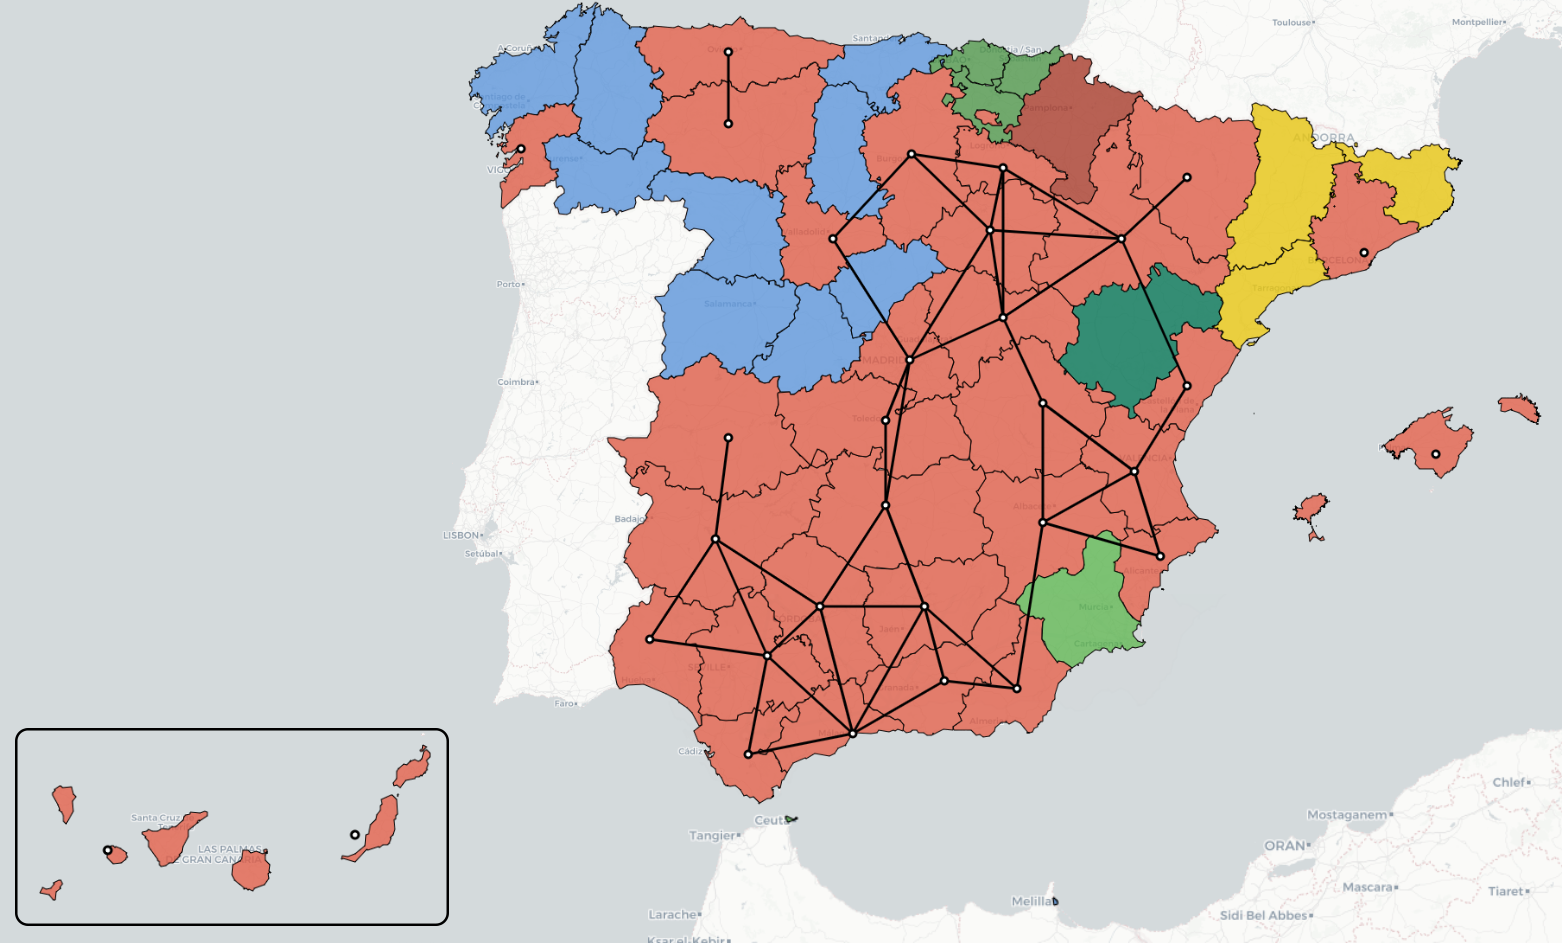
\includegraphics[width=\textwidth]{include/figuras/mapaWikipedia.png} 
	\caption{Filtraciones del complejo de Vietoris-Rips con vértices en las coordenadas dadas por Wikipedia de las provincias donde el PSOE ganó en las elecciones generales del noviembre de 2019.}
	\label{ref:mapaWiki}
\end{subfigure}
\begin{subfigure}[b]{\textwidth}
	\centering
	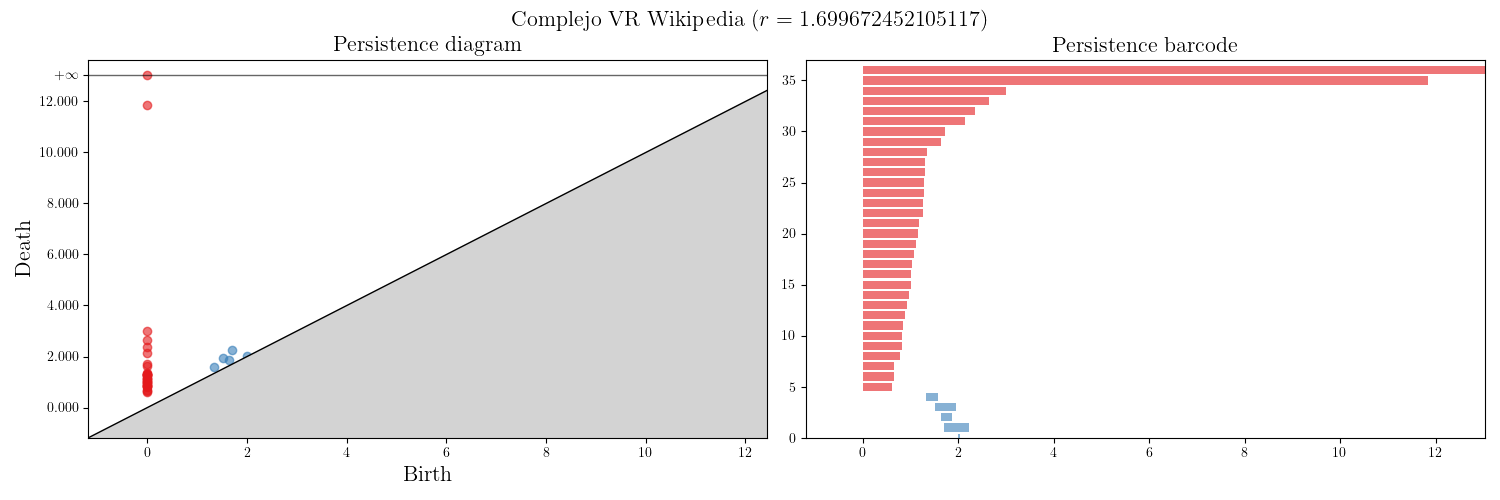
\includegraphics[width=\textwidth]{../code/output/ejemploMapa.png} 
	\caption{Diagrama de persistencia y código de barras asociado a las filtraciones de dicho complejo de Vietoris-Rips.}
	\label{ref:persMapaWiki}
\end{subfigure}
\caption{Estudio de la persistencia sobre los datos originales.}
\label{ref:figMapaWiki}
\end{figure} 
\vspace*{\fill}
\newpage
\begin{figure}[!ht]
\centering
\begin{subfigure}[b]{\textwidth}
	\centering
	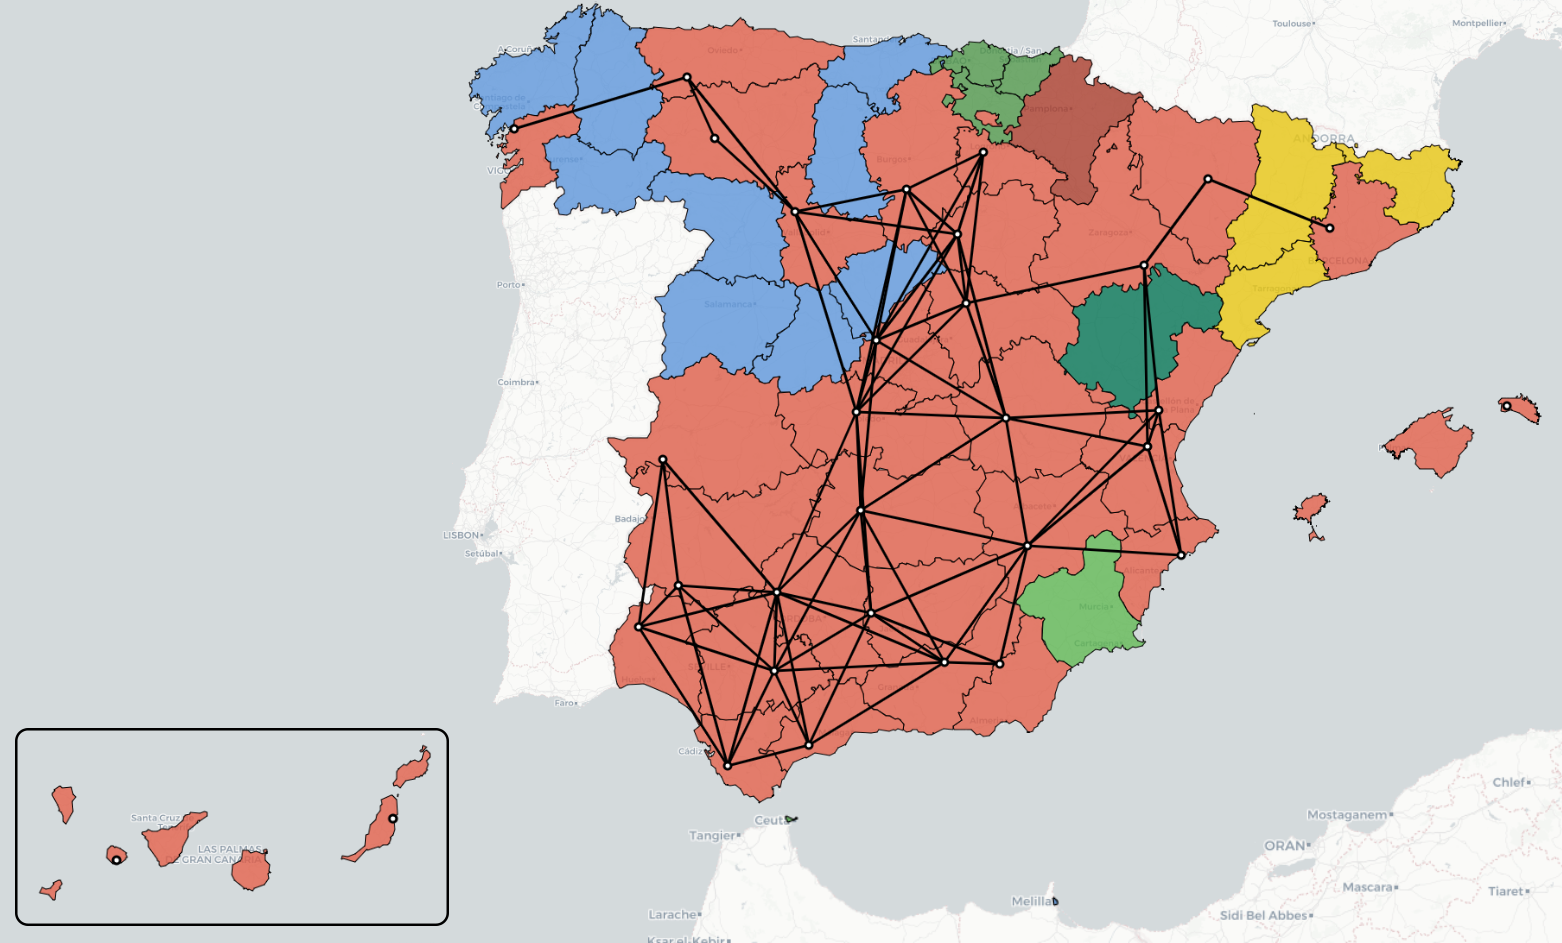
\includegraphics[width=\textwidth]{include/figuras/mapaRandom.png} 
	\caption{Filtración del complejo de Vietoris-Rips con vértices en unas coordenadas aleatorias sobre las provincias donde el PSOE ganó en las elecciones generales del noviembre de 2019.}
	\label{ref:mapaRandom}
\end{subfigure}
\begin{subfigure}[b]{\textwidth}
	\centering
	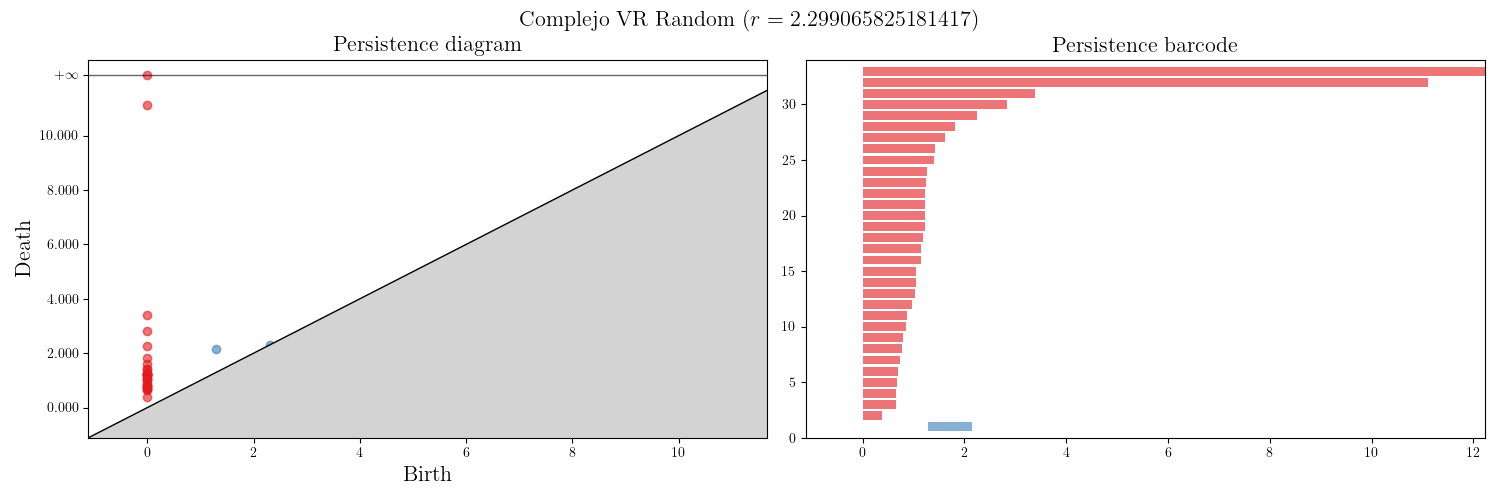
\includegraphics[width=\textwidth]{../code/output/ejemploMapa2.png} 
	\caption{Diagrama de persistencia y código de barras asociado a las filtraciones de dicho complejo de Vietoris-Rips.}
	\label{ref:persMapaRandom}
\end{subfigure}
\caption{Estudio de la persistencia al aplicar ruido a los datos.}
\label{ref:figMapaRandom}
\end{figure}

Como hemos podido observar en las figuras \ref{ref:persMapaWiki} y \ref{ref:persMapaRandom}, los diagramas de persistencia son muy cercanos. Esto se observa también al calcular las distancias bottleneck. Cabe destacar que los diagramas de persistencia nos dan a pensar que nuestro mapa (restringido a las provincias que ganó el PSOE) sólo tiene dos componentes conexas, la zona peninsular (península y baleares) y las islas canarias, sin embargo, sería más correcto si pudieramos obtener 3 componentes conexas  bien identificables como mínimo. Siguiendo el estudio de las componentes conexas también se muestran unas clases que sobreviven un poco más que el resto, las cuales hacen referencia a Pontevedra y Barcelona, las cuales no se encuentran conectadas con el bloque central.

Desde el punto de vista de los agujeros podemos observar que en ambos casos se muestra a Teruel como agujero, sin embargo en el caso de los puntos obtenidos de las coordenadas de Wikipedia la clase de homología de dimensión 1 que más tiempo sobrevive realmente no representa ninguna isla de voto, simplemente es producto del complejo de Vietoris-Rips, lo que nos indica (al igual que se observa en \cite{votosArticulo}) que este tipo de complejo simplicial no sea el más apropiado para esta tarea.

Desde el punto de vista de la estabilidad podemos observar que la distancia bottleneck es inferior a la distancia Hausdorff entre los conjuntos de puntos, dando lugar a la robustez que nos garantiza el \emph{Teorema de estabilidad}.

\begin{minipage}{\linewidth}
\consola{Ejemplo3}
\end{minipage}